%%% Article: Software System for Data Acquisition and Analysis Operating the ATLAS-TPX Network
%%% Authors: Petr Manek, Jakub Begera
%%% Copyright (c) 2017 IEAP CTU


\section{\label{sec:dal}Visualization Application}
Processed data can be examined directly from the ROOT files or by means of the Data Visualization Application. \cite{Manek2016} This application features a web interface capable of displaying frames given specific detector, date and time. In addition, the application is capable of plotting fluxes of characteristic traces in specified time periods. See Fig. \ref{fig:visualizer}.

Since the data is visualized on client-side using modern rendering techniques, the application can also offer basic data operations such as cluster filtering, pixel masking, data aggregation and integral view.

The application serves mainly as a tool of manual inspection of the network operation history. It is openly available to the scientific community upon request.

\begin{figure*}[tbp]
  \centering
  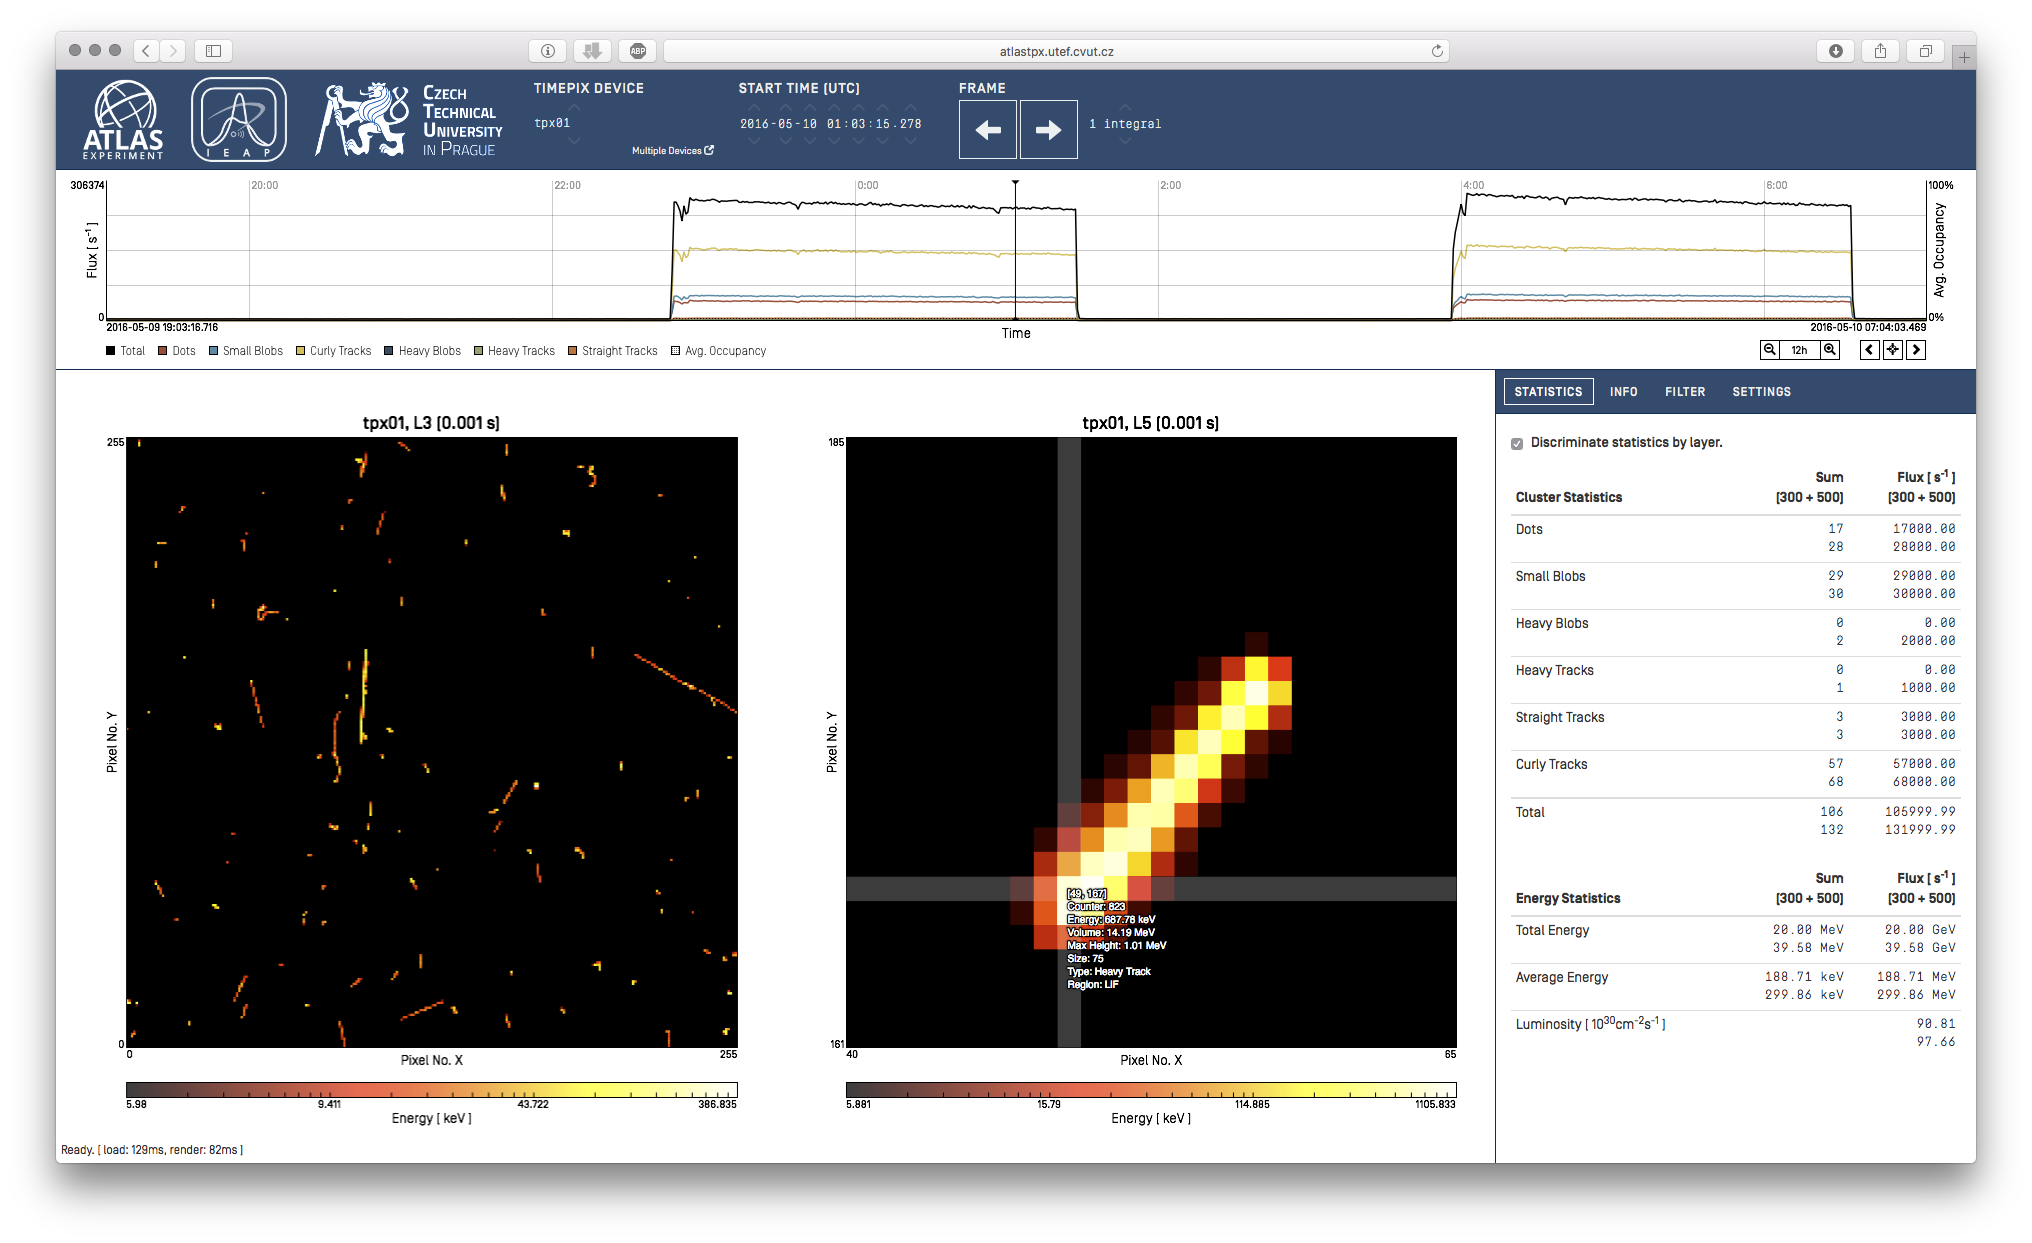
\includegraphics[clip, width=\textwidth, angle = 0 ]{Plots/screen-tpx01-crosshair-zoomed.png}
  \caption {Screenshot of the Data Visualization Application. \cite{Manek2016} Top chart shows occupancy and flux of characteristic traces (differentiated by colors) in frames of specified time range, the vertical line in the middle indicates a selected point in time. Bottom charts show pixel matrices from both TPX sensor layers of a specified detector at the selected time point, the position of the mouse cursor (in the right matrix) is highlighted, showing more information about the trace underneath. Such information includes results of morphological classification, converter region, size, volume, etc. Right sidebar shows a table with characteristic trace counts and fluxes for the displayed frame and interactive filter control interface, which is capable of formulating a custom predicate from cluster and pixel data. The application is available online at \url{https://tpx-visualizer.cern.ch/}, access is granted upon request.}
  \label{fig:visualizer}
\end{figure*}
